\documentclass[tikz,border=6pt]{standalone}
\usepackage[T1]{fontenc}
\usepackage[utf8]{inputenc}
\usepackage{pgfplots}
\usepgfplotslibrary{groupplots}
\usetikzlibrary{calc}
\pgfplotsset{compat=1.18}
\begin{document}
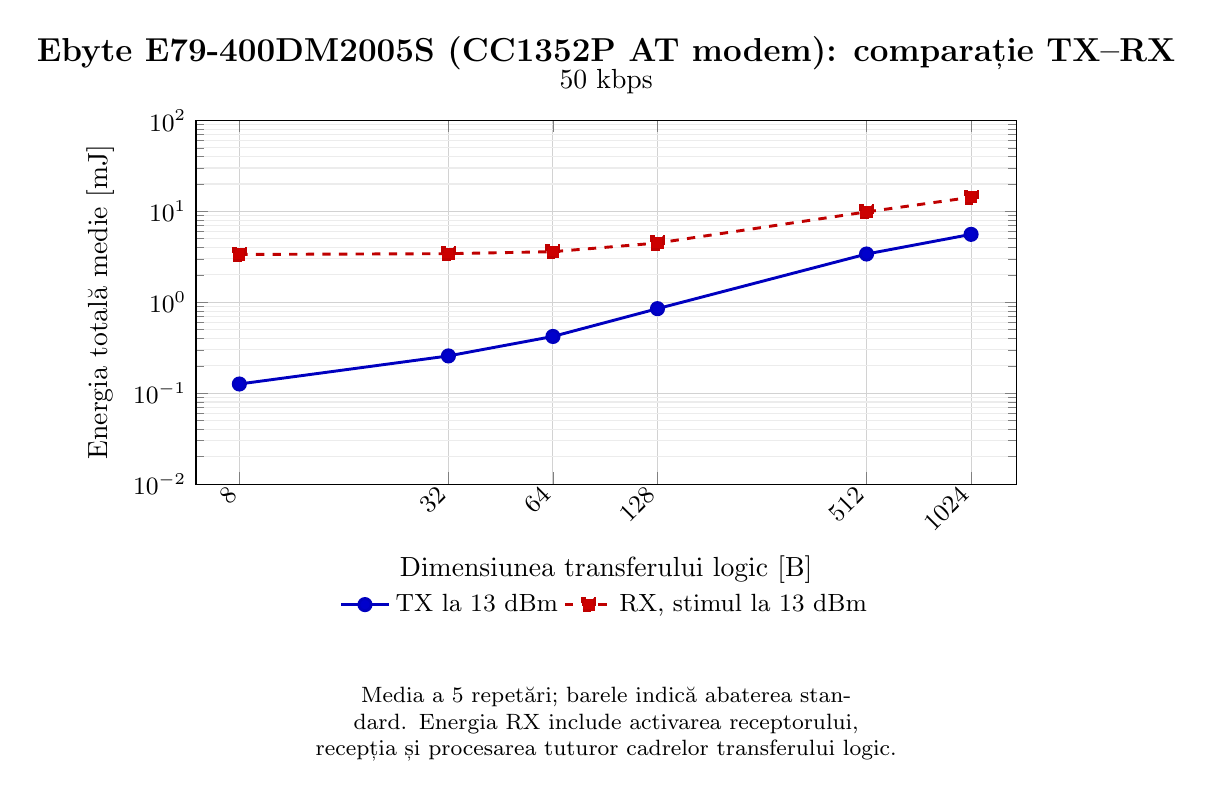
\begin{tikzpicture}
\begin{groupplot}[/pgf/number format/use comma,
  group style={group size=1 by 1, horizontal sep=1.15cm},
  width=12.0cm, height=6.2cm,
  xmode=log, log basis x={2}, ymode=log, log basis y={10},
  ymin=0.01, ymax=100,
  xmin=6, xmax=1382.4,
  xtick={8,32,64,128,512,1024}, xticklabels={8,32,64,128,512,1024},
  x tick label style={rotate=45, anchor=east, font=\small},
  y tick label style={font=\small},
  grid=both, minor grid style={gray!15}, major grid style={gray!35},
  xlabel={Dimensiunea transferului logic [B]},
  every axis plot/.append style={line width=1.05pt},
  error bars/error bar style={line width=0.35pt},
  legend style={font=\small, draw=none, fill=none,
    at={(0.5,-0.27)}, anchor=north, legend columns=2},
]
\nextgroupplot[title={50 kbps}, ylabel={Energia totală medie [mJ]}]
\addplot+[blue!75!black, solid, mark=*, mark size=2.2pt,
  error bars/.cd, y dir=both, y explicit,
] coordinates {
  (8,0.126110346) +- (0,0.0046818786)
  (32,0.256786687) +- (0,0.00404649346)
  (64,0.420437186) +- (0,0.0199228743)
  (128,0.849975348) +- (0,0.0200749542)
  (512,3.39264958) +- (0,0.035218882)
  (1024,5.58319835) +- (0,0.0162436864)
};
\addlegendentry{TX la 13 dBm}
\addplot+[red!75!black, dashed, mark=square*, mark size=2.2pt,
  error bars/.cd, y dir=both, y explicit,
] coordinates {
  (8,3.35532953) +- (0,0.0430443526)
  (32,3.42230825) +- (0,0.0451421625)
  (64,3.60030454) +- (0,0.0943441492)
  (128,4.48277937) +- (0,0.10553414)
  (512,9.86210225) +- (0,0.077230891)
  (1024,14.2673615) +- (0,0.0258167812)
};
\addlegendentry{RX, stimul la 13 dBm}
\end{groupplot}
\node[font=\bfseries\large] at ($(group c1r1.north)+(0,0.85cm)$)
  {Ebyte E79-400DM2005S (CC1352P AT modem): comparație TX--RX};
\node[font=\footnotesize, align=center, text width=12cm]
  at ($(group c1r1.south)+(0,-3.05cm)$)
  {Media a 5 repetări; barele indică abaterea standard. Energia RX include activarea receptorului,\\
   recepția și procesarea tuturor cadrelor transferului logic.};
\end{tikzpicture}
\end{document}
